\documentclass[a4paper,10pt]{article}

\input{packages.tex}
\usetheme{metropolis}

\usepgfplotslibrary{dateplot}

\lstset{
  basicstyle=\ttfamily,
  mathescape
}

\title{Reavaliação}
\posttitle{\end{center}}

\begin{document}

\maketitle

\emergencystretch 3em

\input{recommendations.tex}

NOME: \rule{.85\textwidth}{0.1mm}

\begin{multicols*}{2}
\setlength{\leftmargini}{0pt}
\begin{enumerate}
  \item (2,5 pt) Um determinado grafo \textit{não direcionado} possui 6 vértices, $V = \{1, 2, 3, 4, 5, 6\}$ e 6 arestas. As arestas conectam sempre dois números pares ou dois números ímpares, nunca um número par com um número ímpar.

  \begin{enumerate}
    \item (0,4 pt) Faça uma representação visual do grafo.
    %    (1)         (2)
    %   /   \       /   \
    % (3)---(5)   (4)---(6)
    \item (0,5 pt) Faça a matriz de adjacência do grafo.
    %   1  2  3  4  5  6
    % 1 0  0  1  0  1  0
    % 2 0  0  0  1  0  1
    % 3 1  0  0  0  1  0
    % 4 0  1  0  0  0  1
    % 5 1  0  1  0  0  0
    % 6 0  1  0  1  0  0
    \item (0,5 pt) Faça as listas de adjacência do grafo.
    % 1->|3||->|5||-> NULL
    % 2->|4||->|6||-> NULL
    % 3->|1||->|5||-> NULL
    % 4->|2||->|6||-> NULL
    % 5->|1||->|3||-> NULL
    % 6->|2||->|4||-> NULL
    \item (0,5 pt) Qual o número de componentes conectados nesse grafo? % Dois.
    \item (0,6 pt) Esse grafo é cíclico? Se sim, especifique quantos ciclos e quais vértices fazem parte de cada ciclo. % Sim. Dois ciclos. 1->3->5->1, 2->4->6->2.
  \end{enumerate}

  \item (3,0 pt) A imagem a seguir representa um \textit{grafo de Franklin}, com 12 vértices e 18 arestas.

  \begin{center}
    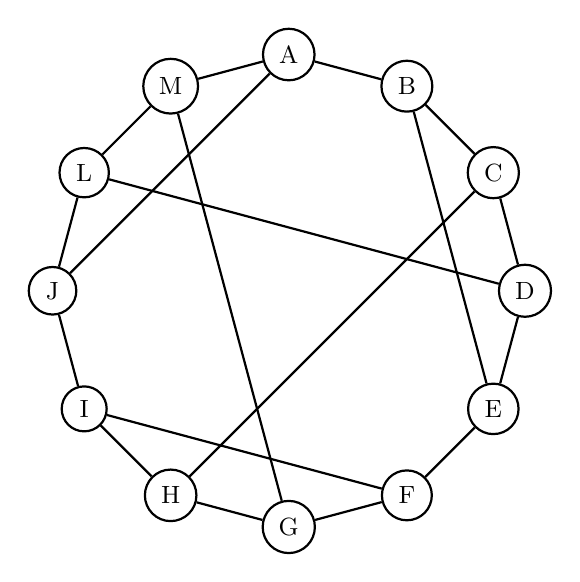
\begin{tikzpicture}[scale=0.75]
      \foreach \x\y in {1/A,2/B,3/C,4/D,5/E,6/F,7/G,8/H,9/I,10/J,11/L,12/M} {
        \node[circle, draw=black, thick] (\y) at ({-\x*30 + 120}:4){\small \y};
      }

      \draw[thick]
        (A) -- (B) --
        (C) -- (D) --
        (E) -- (F) --
        (G) -- (H) --
        (I) -- (J) --
        (L) -- (M) --
        (A);

      \draw[thick] (B) -- (E);
      \draw[thick] (F) -- (I);
      \draw[thick] (J) -- (A);
      \draw[thick] (C) -- (H);
      \draw[thick] (D) -- (L);
      \draw[thick] (G) -- (M);
    \end{tikzpicture}
  \end{center}

  \begin{enumerate}
    \item (1,3 pt) Faça uma BFS no grafo e obtenha a relação de parentesco entre os vértices, começando a partir do vértice A e explorando em ordem alfabética. Desenhe essa relação em um formato de árvore. Lembre-se de usar uma fila para organizar a exploração.
    %            _________(A)____
    %           /          |     \
    %        _(B)_        (J)    (M)
    %       /     \      /   \    |
    %     (C)     (E)  (I)   (L) (G)
    %    /   \     |
    %  (D)   (H)  (F)
    %
    %  Fila: A B J M C E I L G D H F
    %  A  B  C  D  E  F  G  H  I  J  L  M
    % -1  A  B  C  B  E  M  C  J  A  J  A
    \item (0,6 pt) De acordo com o resultado da letra (a), qual é o caminho com menos arestas entre os vértices A e F?
    % A -> B -> E -> F
    \item (1,1 pt) Esse grafo é bipartido? Se sim, desenhe-o com os vértices coloridos. Caso contrário, mostre em que momento da BFS ocorre um conflito na hora de preencher as cores.
    % Sim.
    % A: P | G: P
    % B: B | H: B
    % C: P | I: P
    % D: B | J: B
    % E: P | L: P
    % F: B | M: B
  \end{enumerate}

  \item (3,0 pt) A matriz de adjacência a seguir representa um grafo \textit{não direcionado} com 6 vértices e 8 arestas.

  \begin{equation*}
    \begin{blockarray}{ccccccc}
      & A & B & C & D & E & F \\
      \begin{block}{c(cccccc)}
        A & 0 & 0 & 0 & 0 & 1 & 1 \\
        B & 0 & 0 & 0 & 0 & 1 & 1 \\
        C & 0 & 0 & 0 & 0 & 1 & 1 \\
        D & 0 & 0 & 0 & 0 & 1 & 1 \\
        E & 1 & 1 & 1 & 1 & 0 & 0 \\
        F & 1 & 1 & 1 & 1 & 0 & 0 \\
      \end{block}
      \end{blockarray}
  \end{equation*}

  \begin{enumerate}
    \item (1,2 pt) Faça uma DFS no grafo, começando a partir do vértice A e explorando em ordem alfabética. Obtenha a relação de parentesco entre os vértices e desenhe essa relação no formato de uma árvore. Lembre-se de usar uma pilha para organizar a exploração.
    %    (A)
    %     |
    %    (E)
    %     |
    %    (B)
    %     |
    %    (F)
    %   /   \
    % (C)  (D)
    \item (0,8 pt) Classifique todas as arestas do grafo.
    % A - E Árvore
    % A - F Retorno
    % B - E Árvore
    % B - F Árvore
    % C - E Retorno
    % C - F Árvore
    % D - E Retorno
    % D - F Árvore
    \item (1,0 pt) Transformando o grafo da questão em um DAG (\textit{grafo direcionado acíclico}), temos a matriz de adjacência a seguir. Dê uma ordenação topológica para esse grafo.
    % D B F E C A
    % D B F E A C
    % D B E F C A
    % D B E F A C
    % B D F E C A
    % B D F E A C
    % B D E F C A
    % B D E F A C
  \end{enumerate}

  \begin{equation*}
    \begin{blockarray}{ccccccc}
      & A & B & C & D & E & F \\
      \begin{block}{c(cccccc)}
        A & 0 & 0 & 0 & 0 & 0 & 0 \\
        B & 0 & 0 & 0 & 0 & 1 & 1 \\
        C & 0 & 0 & 0 & 0 & 0 & 0 \\
        D & 0 & 0 & 0 & 0 & 1 & 1 \\
        E & 1 & 0 & 1 & 0 & 0 & 0 \\
        F & 1 & 0 & 1 & 0 & 0 & 0 \\
      \end{block}
      \end{blockarray}
  \end{equation*}

  \item (1,5 pt) Encontre a árvore geradora mínima do grafo a seguir usando o algoritmo de Prim, começando a partir do vértice A. Para arestas de mesmo peso, dê prioridade àquela que apareça primeiro na ordem alfabética. Escreva na sua resposta a ordem em que você visitou cada aresta da árvore. Desenhe a árvore no mesmo formato do grafo.
  % A - D 1
  % A - G 2
  % D - E 3
  % E - H 3
  % H - F 4
  % E - B 7
  % B - C 6
  %
  % (A)      (B)
  %  | \    /  \
  %  |  \ (C)   \
  %  |   \       \
  %  |  (D)-----(E)
  %  |          /
  %  |    (F)  /
  %  |      \ /
  % (G)     (H)
  %

  \begin{center}
  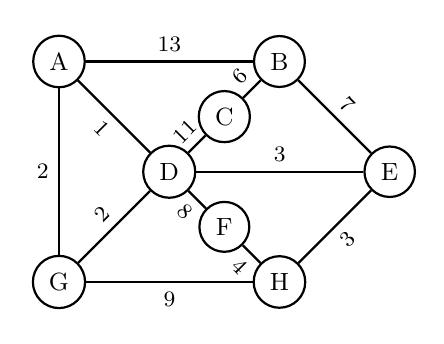
\begin{tikzpicture}[scale=0.7]
    \node[circle, draw=black, thick](A) at (0.00, 4.00){\small A};
    \node[circle, draw=black, thick](B) at (4.00, 4.00){\small B};
    \node[circle, draw=black, thick](C) at (3.00, 3.00){\small C};
    \node[circle, draw=black, thick](D) at (2.00, 2.00){\small D};
    \node[circle, draw=black, thick](E) at (6.00, 2.00){\small E};
    \node[circle, draw=black, thick](F) at (3.00, 1.00){\small F};
    \node[circle, draw=black, thick](G) at (0.00, 0.00){\small G};
    \node[circle, draw=black, thick](H) at (4.00, 0.00){\small H};

    \draw[thick] (A) -- node[anchor=east](){\footnotesize 2} (G);
    \draw[thick] (A) -- node[anchor=south](){\footnotesize 13} (B);
    \draw[thick] (G) -- node[anchor=north](){\footnotesize 9} (H);
    \draw[thick] (A) -- node[anchor=north,rotate=-45](){\footnotesize 1} (D);
    \draw[thick] (G) -- node[anchor=south,rotate=45](){\footnotesize 2} (D);
    \draw[thick] (D) -- node[anchor=south](){\footnotesize 3} (E);
    \draw[thick] (B) -- node[anchor=south,rotate=-45](){\footnotesize 7} (E);
    \draw[thick] (H) -- node[anchor=north,rotate=45](){\footnotesize 3} (E);
    \draw[thick] (B) -- node[anchor=south,rotate=45](){\footnotesize 6} (C);
    \draw[thick] (C) -- node[anchor=south,rotate=45](){\footnotesize 11} (D);
    \draw[thick] (H) -- node[anchor=north,rotate=-45](){\footnotesize 4} (F);
    \draw[thick] (F) -- node[anchor=north,rotate=-45](){\footnotesize 8} (D);
  \end{tikzpicture}
  \end{center}

\end{enumerate}
\end{multicols*}
\end{document}
